\section{Part I: Data Cleaning and Preprocessing (for dataset A)}
\subsection{Detecting Issues in the dataset}
For this part of the assignment, the dataset had to be analyzed first as part of the preprocessing step to detect issues such as missing values and outliers. There was found to be a 124053 missing values and 14622 outliers in the dataset. Outliers were found by first finding the standard deviation of each feature and then using each standard deviation to find values in that specific feature that vary by more than 3 standard deviations. 

\subsection{Fixing Issues}
Before replacing the missing values with the mean, the outliers had to be checked first since the mean would be effected by those outliers. There were over 14000 data points (makes ~0.9 percent of the entire data) that vary from the features mean by over 3 standard deviations. Since the nature of the experiment is not well defined, those outliers are assumed to be noise detected by the motion sensors. After the detection of the outliers, they were replaced with the mean of each feature. Final step was to replace all the missing values denoted by NA with the mean of each feature after the outliers were taken care of. 

\subsection{Normalizing Data}



Figure~\ref{fig:fig1} shows the comparison between histogram plots of feature 9 and 24 before and after normalization

%%%%%%%%%%%%%%%%%%%%%%%%%%%%%%%%%%%%%%%%%%%%%%%%%%%%%%%%%%%%%%%%%%%
%
% Commands to include a figure:
%
%%%%%%%%%%%%%%%%%%%%%%%%%%%%%%%%%%%%%%%%%%%%%%%%%%%%%%%%%%%%%%%%%%%

\begin{figure}[!ht]
 \centering
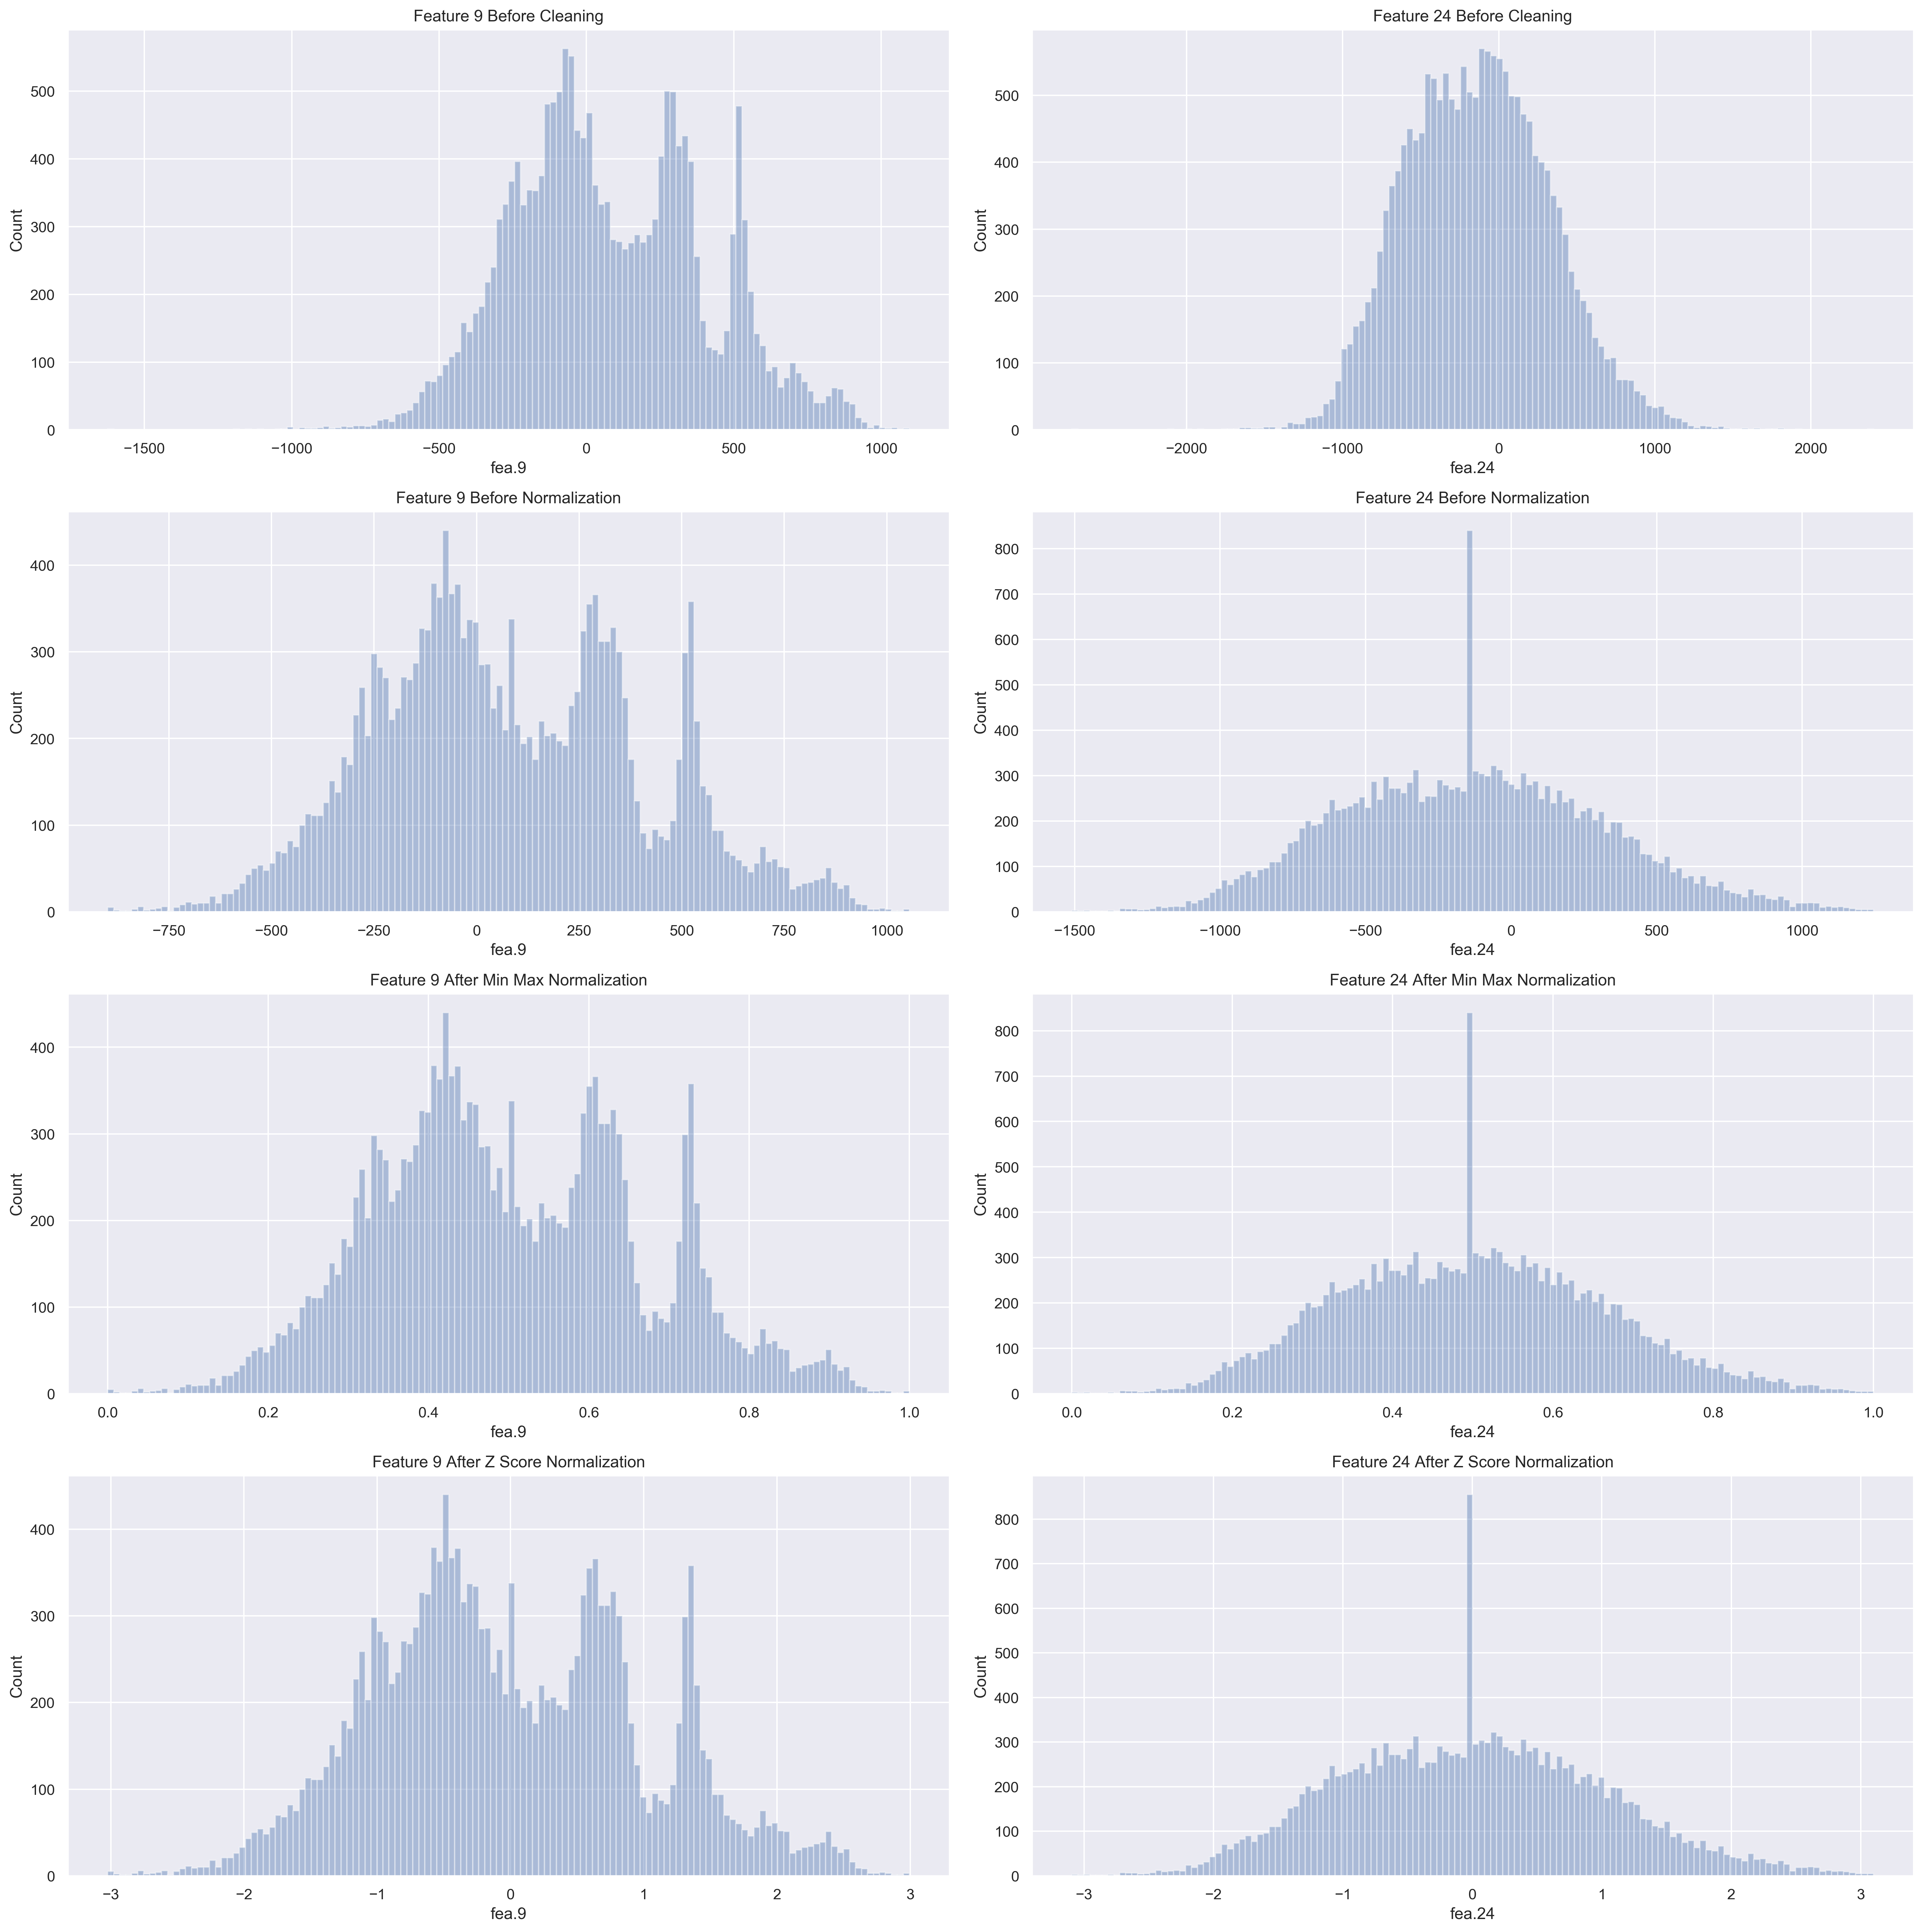
\includegraphics[width=6.1in]{assignment1/1-3-histograms.png}
\caption{\label{fig:fig1}histogram plots of feature 9 and 24 before and after normalization}
\end{figure}
